\documentclass[a4paper]{article}
\usepackage[utf8]{inputenc}
\usepackage[english]{babel}
\usepackage[T1]{fontenc}
\usepackage{lmodern}
\usepackage{fullpage}
\usepackage{amsmath}
\usepackage{graphicx}
\usepackage{framed}
\usepackage{listings}
\usepackage{placeins}
\usepackage{subcaption}
\usepackage{array}
\usepackage[justification=centering]{caption}

\author{Théotime Grohens}
\title{Introduction to Computer Vision: \\ Assignment 4: Essential matrix}

\begin{document}

\maketitle

\section*{Question 1}

The mean distance without normalization is 207.70.

Figures:

\begin{figure}[h]
\begin{subfigure}{0.5\textwidth}
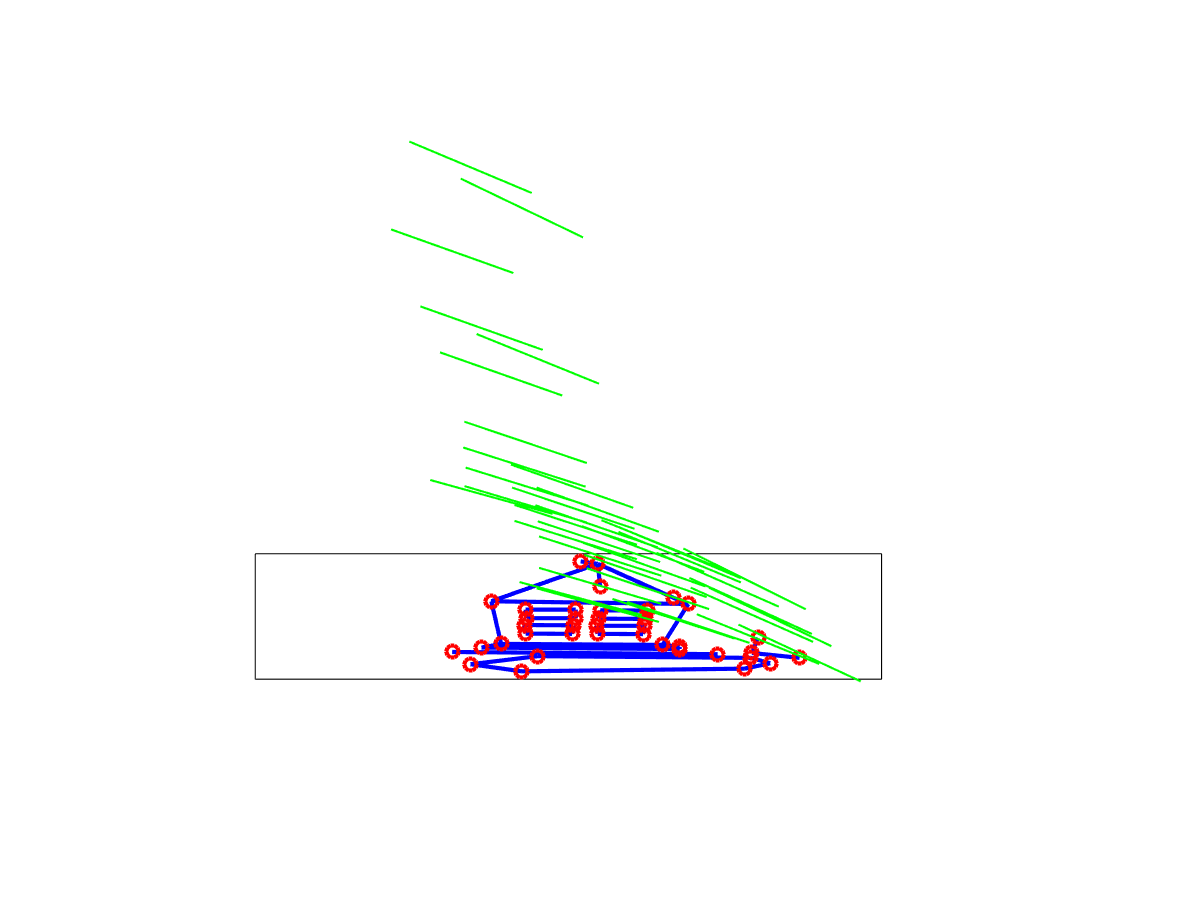
\includegraphics[width=\textwidth]{epi1.png}
\end{subfigure}
\begin{subfigure}{0.5\textwidth}
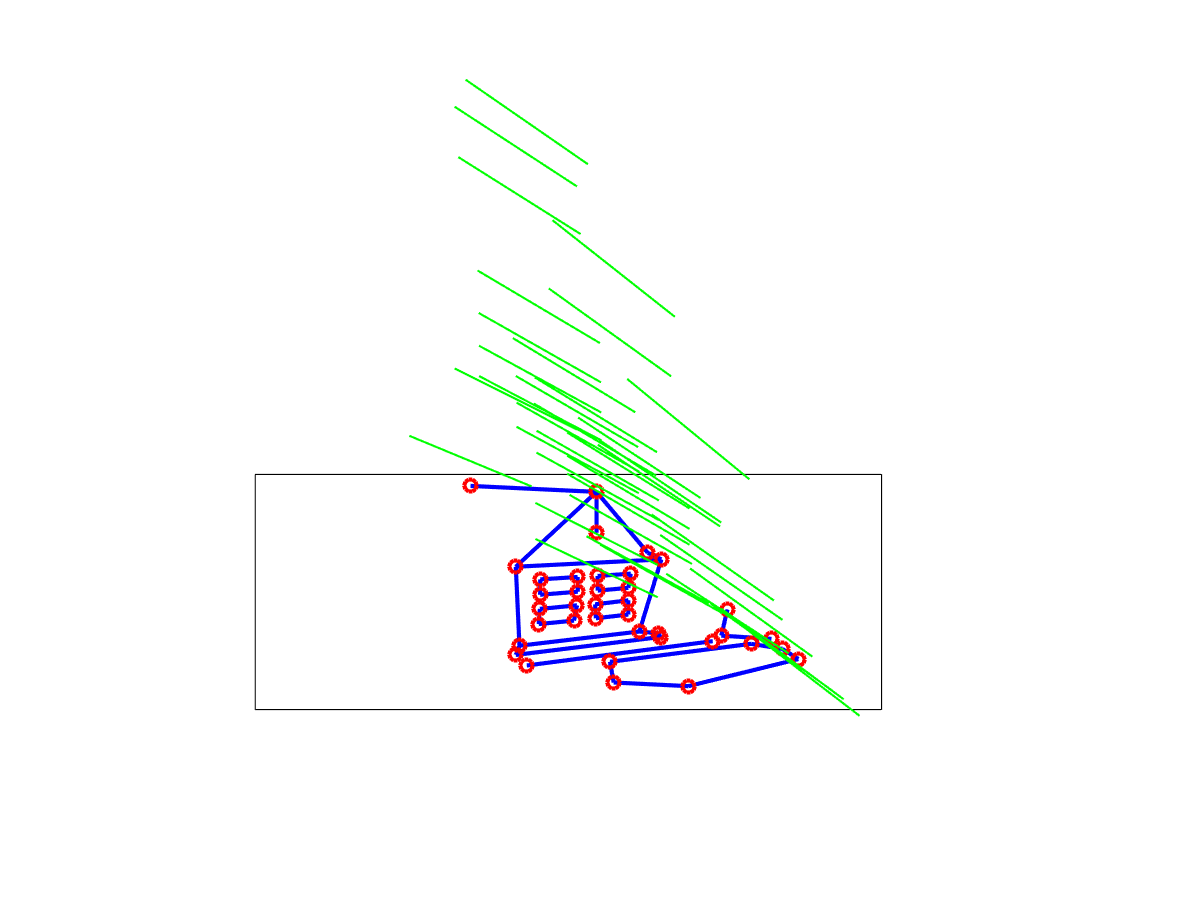
\includegraphics[width=\textwidth]{epi2.png}
\end{subfigure}
\end{figure}

\section*{Question 2}

The mean distance with normalization is 364.24.

Figures:

\begin{figure}[h]
\begin{subfigure}{0.5\textwidth}
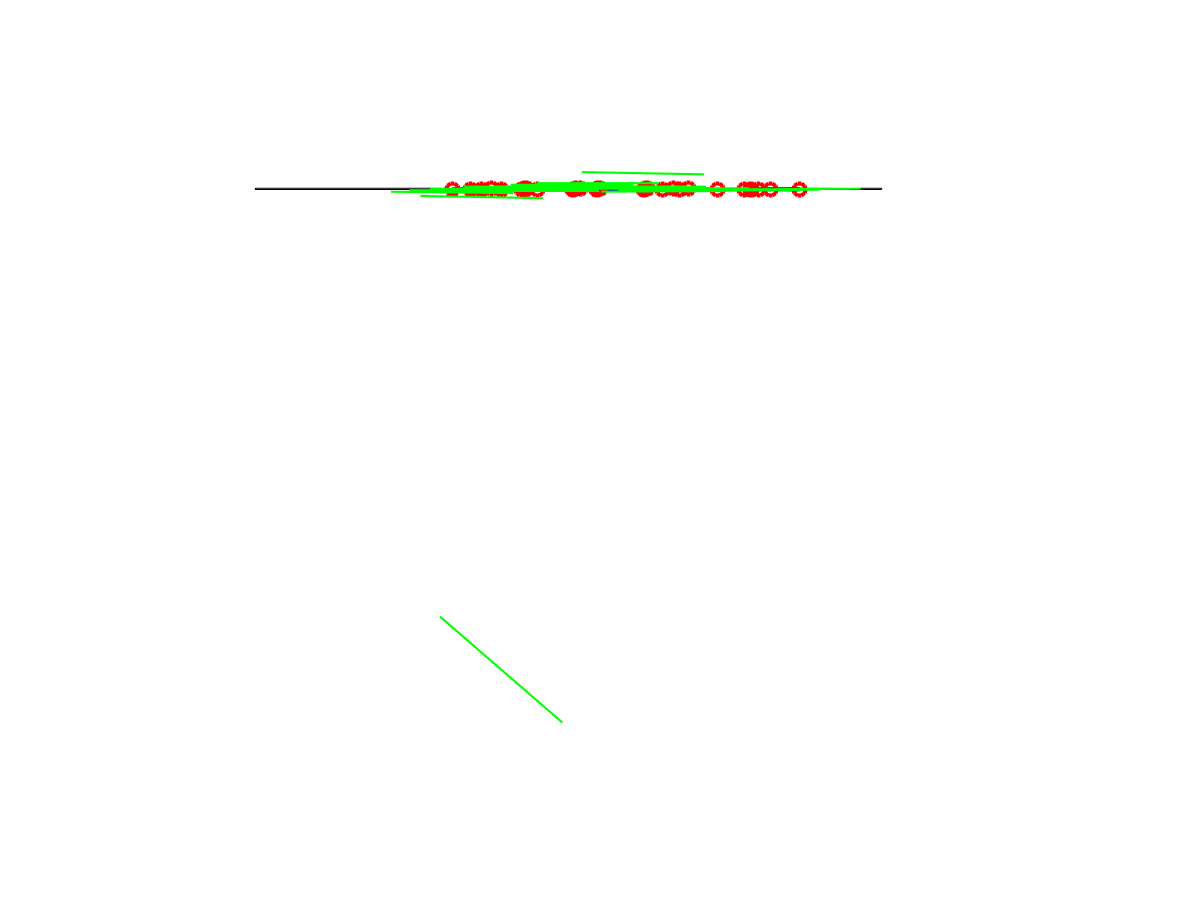
\includegraphics[width=\textwidth]{epi1H.png}
\end{subfigure}
\begin{subfigure}{0.5\textwidth}
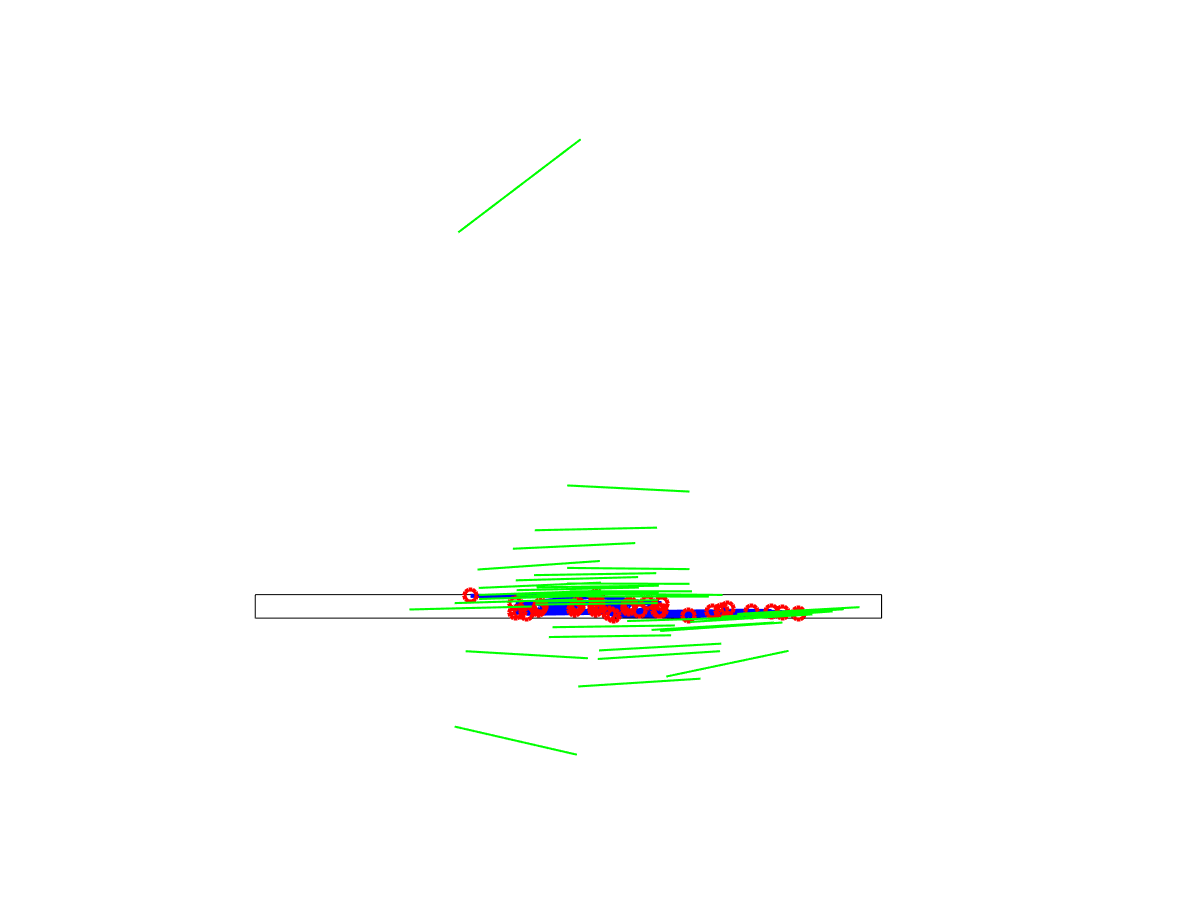
\includegraphics[width=\textwidth]{epi2H.png}
\end{subfigure}
\end{figure}

\end{document}